\documentclass[12pt]{article}
\usepackage[margin=1.25in]{geometry}
\usepackage{titling}
\setlength{\droptitle}{-6\baselineskip}
\pagenumbering{gobble}

\usepackage{graphicx}
\graphicspath{{./}}

\usepackage{enumitem}
\usepackage{tipa}


\title{LING 285 -- Final Project Part 1}
\author{D. Choi}
\date{2022-02-09}

\begin{document}


\maketitle

\paragraph{1.}
\begin{enumerate}[label=\textbf{\alph*.}]
    \item \textbf{\textipa{[\textesh]}}: vocal cords apart, past the alveolar ridge, velum raised, tract almost closed
    \item \textbf{\textipa{[n]}}: vold cords together, at the alveolar ridge, velum lowered, tract fully closed
    \item \textbf{\textipa{[k]}}: vocal cords apart, at the velum, velum raised, tract fully closed
    \item \textbf{\textipa{[g]}}: vocal cords together, at the velum, velum raised, tract fully closed
    \item \textbf{\textipa{[\texttheta]}}: vocal cords apart, at the teeth, velum raised, tract almost closed
    \item \textbf{\textipa{[b]}}: vocal cords together, at the lips, velum raised, tract fully closed
\end{enumerate}

\paragraph{2.}
\begin{enumerate}[label=\textbf{\alph*.}]
    \item \textbf{\textipa{[\textsci]}}: high and front
    \item \textbf{\textipa{[o]}}: middle and back
    \item \textbf{\textipa{[\textscripta]}}: low and back
    \item \textbf{\textipa{[e]}}: middle and front
\end{enumerate}

\paragraph{3.}
See \texttt{[i].wav}.

\paragraph{4.}
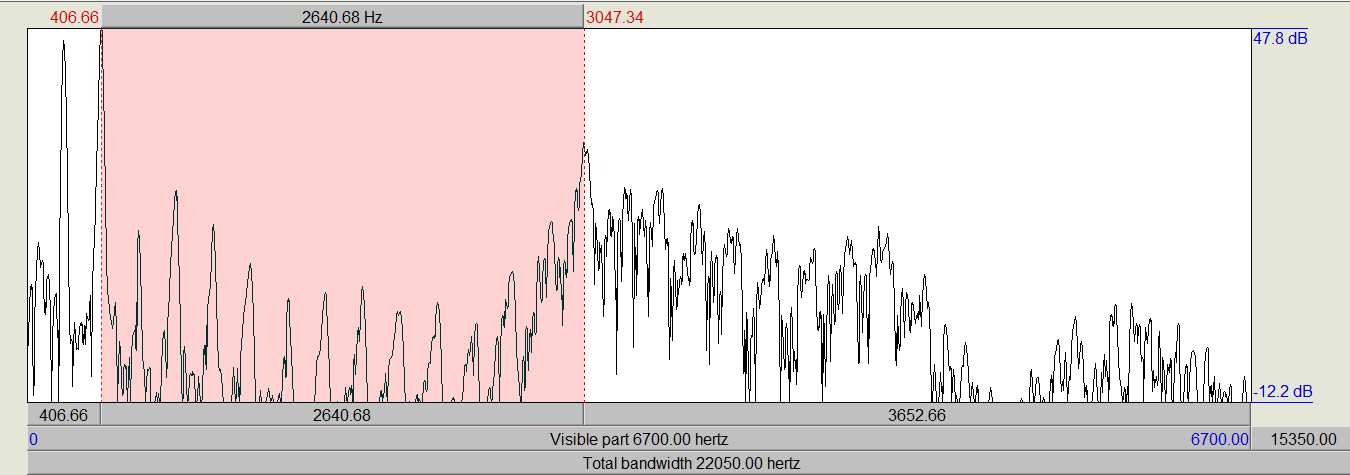
\includegraphics[width=0.9\textwidth]{[i]-spectrum.png}

\paragraph{5.}
\begin{enumerate}[label=\textbf{\alph*.}]
    \item \textbf{Fundamental Frequency}: 203.12 Hz
    \item \textbf{F1}: 406.66 Hz
    \item \textbf{F2}: 3047.34 Hz
\end{enumerate}

\end{document}
